%!TEX encoding = UTF-8 Unicode
\documentclass{slideclass}

\setbeamertemplate{footline}[frame number]
\title[Open Source Software Requirements Engineering (OSSRE)]
{\textbf{A Contribution Management Framework}\\{\small for Firms
Engaged in Open Source Software Ecosystems}}
\subtitle{\small-- a research preview}
\author{Johan Linåker, Björn Regnell}
\institute{Lund University}
\date{2017 Feb 28 \\ 
\vspace{2em}
{\footnotesize This presentation is available here: \url{http://github.com/bjornregnell/ossre}}
}


\usepackage[backend=bibtex,style=ieee,citestyle=authoryear]{biblatex}
\addbibresource{bibliography_master}
\setbeamerfont{footnote}{size=\tiny}
\begin{document}


\frame{\titlepage}
\frame{\tableofcontents}

\section{Research goal}
\begin{Slide}{Research goal}
\begin{itemize}
\item This major force is \Alert{revolutionizing} software business:\pause
\begin{itemize}
\item[] \Emph{Open Source Software} (OSS)\pause
\end{itemize}
\item ...so this is a major research area for the future:\pause
\begin{itemize}
\item[] \Emph{Open Source Software Requirements Engineering}\pause
\end{itemize}
\end{itemize}
\vspace{1em}

$\rightarrow$ Our research \Alert{goal} and \Emph{focus}:\\
\begin{shaded}
\Alert{Deep understanding} of, and \Alert{effective support} for: \\
\Emph{Contribution management} in OSSRE
\end{shaded}



\end{Slide}

\section{Background}%%%%%%%%%%%%%%%%%%%%%%%%%

\begin{Slide}{Background}\SlideFontSmall
\begin{minipage}{0.29\textwidth}
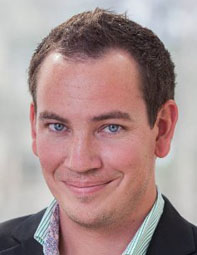
\includegraphics[width=0.8\textwidth]{img/Johan_Linaker_197}

\footnotesize Johan Linåker
\end{minipage}
\begin{minipage}{0.65\textwidth}
Johan Linåker's \Emph{licentiate thesis}:
\begin{itemize}
\item \textbf{''Towards Strategic Support for
Requirements Engineering in Open
Source Software Ecosystems
\\-- What to reveal, when and to whom?''}
\item[] \url{http://cs.lth.se/johan-linaaker/}
\item Systematic literature review on Open Innovation with OSS
\item Network analysis of stakeholder contributions in OSS repos

\end{itemize}
On-going \Alert{doctoral thesis} project:
\begin{itemize}
\item Contribution Management Framework
\end{itemize}
\end{minipage}
{\footfullcite{linaaker2016firms}}
\end{Slide}



\begin{Slide}{Open Innovation and Open Source Software}
Open Innovation modelled as a funnel with permeable border:
{\footfullcite{chesbrough2006researching}}

\vspace{1em}
\begin{minipage}{0.59\textwidth}
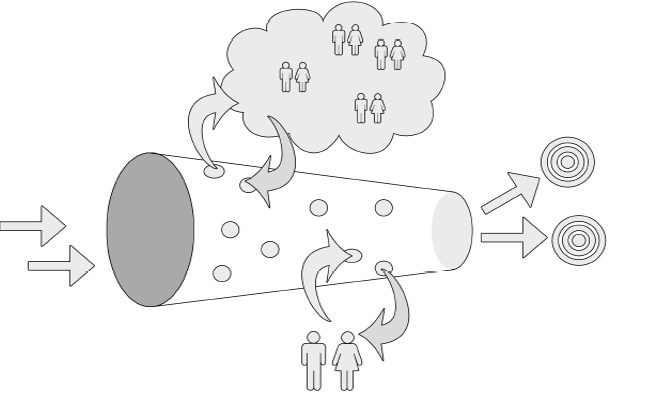
\includegraphics[width=0.95\textwidth]{img/oi}
\end{minipage}
\begin{minipage}{0.4\textwidth}
\SlideFontSmall\pause
\begin{itemize}
\item RE process complexity:
\begin{itemize}\SlideFontSmall
\item Internal RE:\\inside the focal firm
\item External RE:\\in the community
\end{itemize}
\end{itemize}
\end{minipage}

{\SlideFontSmall\pause\vspace{2em}OSS is a major approach to Open Innovation (OI) in the software industry.\vspace{1em}}
\end{Slide}


\begin{Slide}{Stakeholder Network Analysis (Apache Hadoop)}
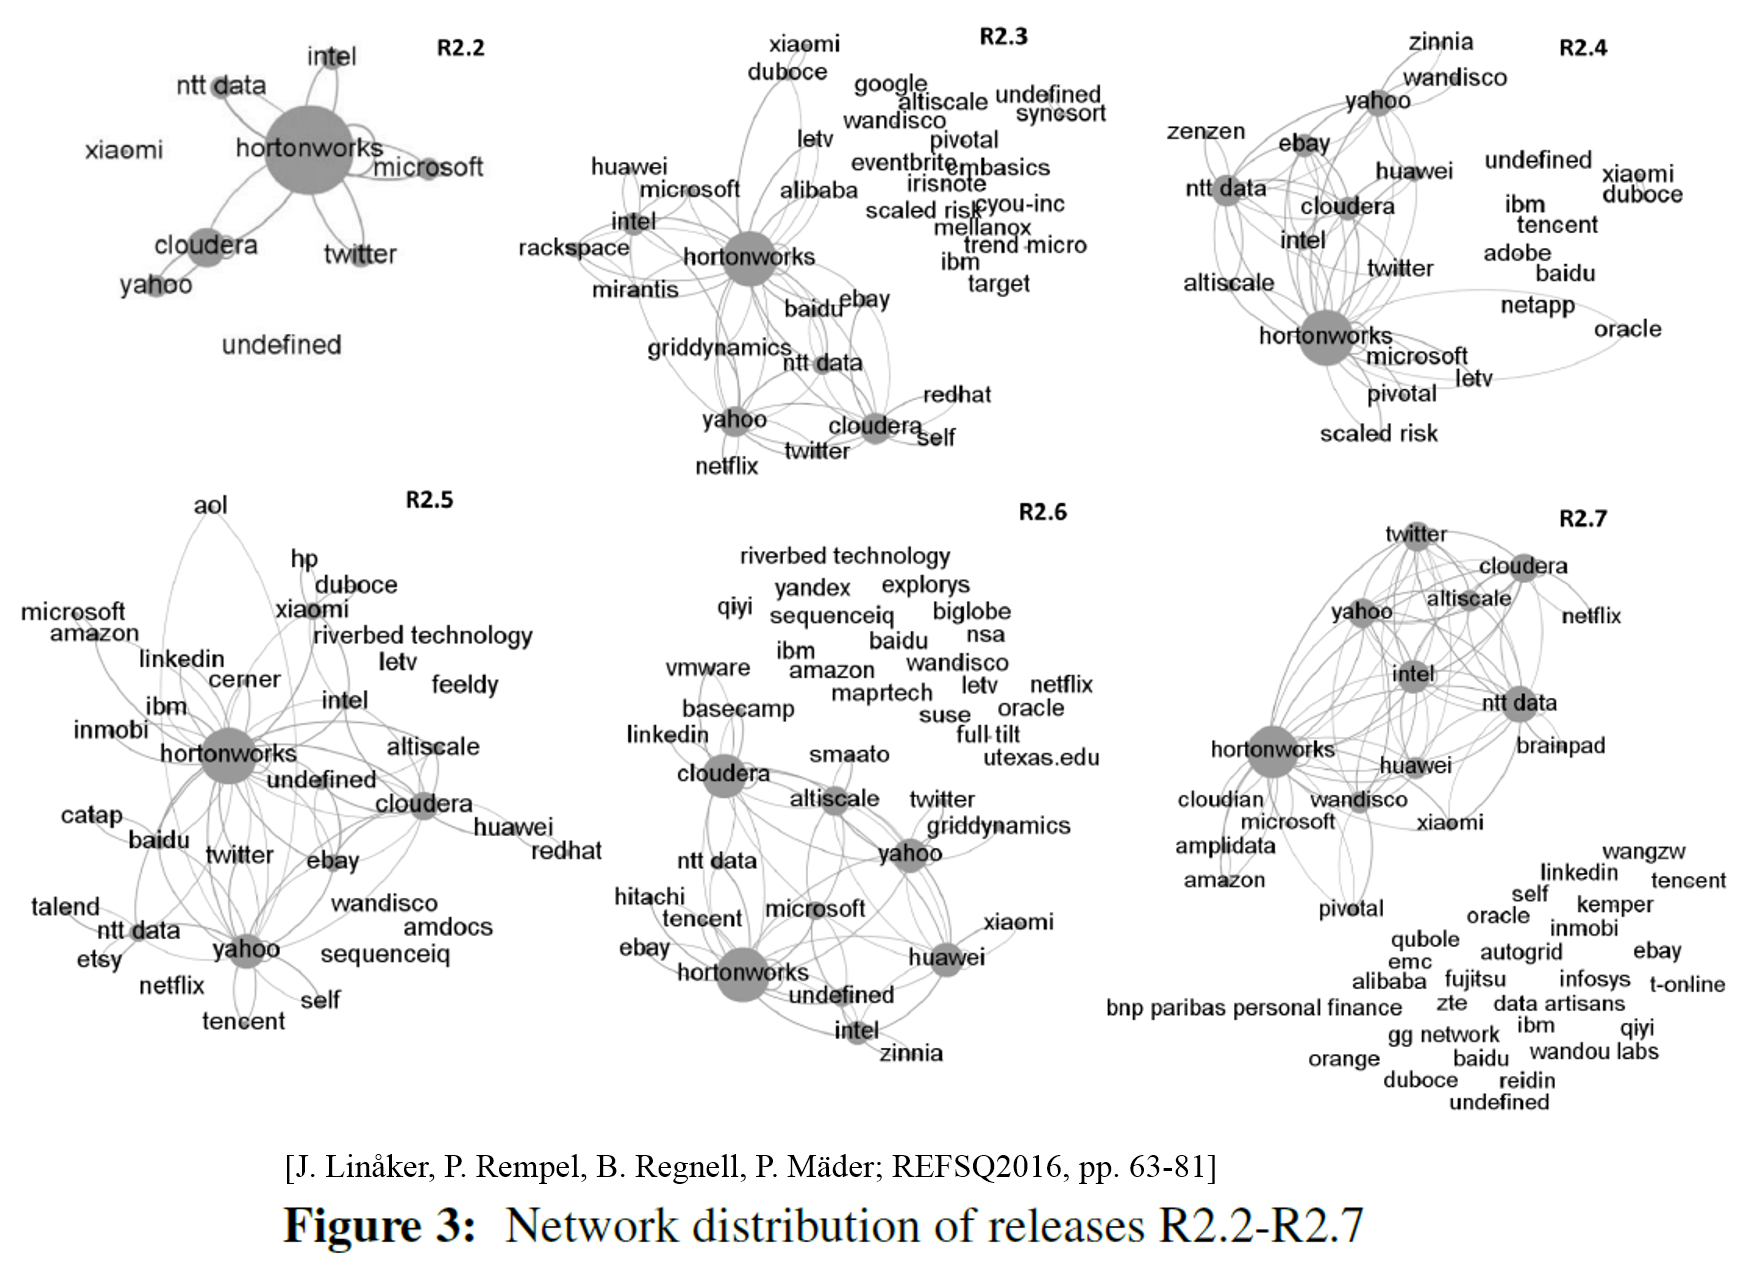
\includegraphics[width=0.90\textwidth]{img/sna}
\end{Slide}

\section{Methodology}%%%%%%%%%%%%%%%%%%%%%%%%
\begin{Slide}{Research methodology}
\begin{itemize}
\item \Emph{Design Science} approach, see Wieringa (2014)\footfullcite{wieringa2014design}
\pause
\item Definition of the \Alert{design problem}: (abbreviated, see paper)
\begin{shaded}
\footnotesize\textbf{Design a framework and tools for OSS \Alert{contribution management} to effectively support product planning in OSSRE.}
\end{shaded}
\pause
\item First iteration:
\begin{itemize}
\item Initial framework based on findings in previous research\footfullcite{munir2015open}\footfullcite{linaaker2016firms}
\item Initial validation: interview with industrial OSS expert 
\end{itemize}
\end{itemize}
\end{Slide}

\section{Results}

\begin{Slide}{Contribution Management Framework}
\begin{shaded}
Stakeholders \hskip0.25em $\rightarrow$ \hskip1.75em Contributions \hskip3em $\rightarrow$ \hskip1em Time Horizons
\end{shaded}

\vspace{1em}Example of questions that the framework may help to answer:
\begin{itemize}
\item Who are the stakeholders in the focal OSS community?
\item Which stakeholders have the same interests as our firm?
\item How to collaborate with the OSS community?
\item What to contribute \& when?
\item Which actions are most important to take in a short-, medium-, and long-term view?
\item ...
\end{itemize}
General goal: How to maximize return-on-investment.
\end{Slide}

\begin{Slide}{Contribution Management Framework}
\begin{shaded}
Stakeholders \hskip0.25em $\rightarrow$ \hskip1.75em Contributions \hskip3em $\rightarrow$ \hskip1em Time Horizons
\end{shaded}

\vspace{1em}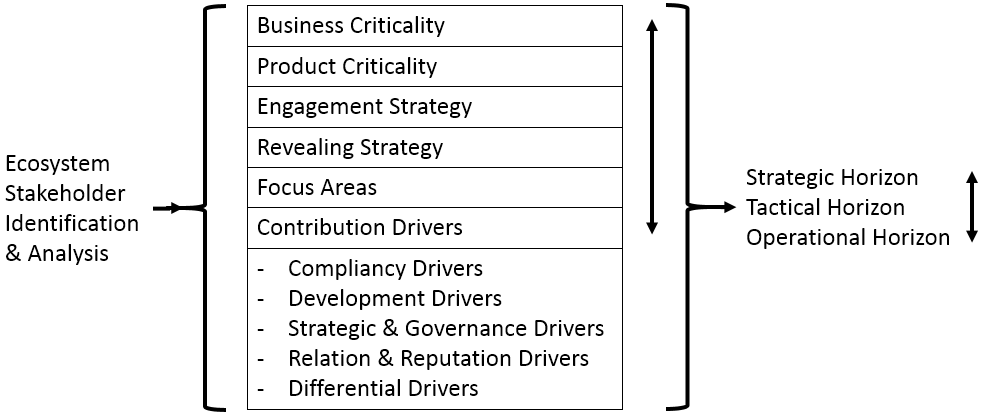
\includegraphics[width=\textwidth]{img/framework_picture}
\end{Slide}

\begin{Slide}{Contribution Management Framework}\SlideFontSmall
Candidate framework ''levels'': from business goals to product contributions
\begin{itemize}
\item \Emph{Business Criticality}: Level of value drawn from the community.
\item \Emph{Product Criticality}: Level of integration with internal product plan/dev.
\item \Emph{Engagement Strategy}: \{Parasitic | Commensalistic | Symbiotic\}
\item \Emph{Revealing Strategy}: Licensing, \{Selective revealing | Full transparency\}
\item \Emph{Focus Areas/Modules}: Selection of product modules to share
\item \Emph{Contribution Drivers}: 
\begin{itemize}\SlideFontSmall
\item Compliancy
\item Development \& Maintenance
\item Strategy \& Governance
\item Relationship \& Reputation
\item Differentiation
\end{itemize}
\end{itemize}
\end{Slide}


\section{Conclusions and future work}
\begin{Slide}{Conclusions and future work}
\begin{itemize}
\item Initial validation indicates utility of the proposed framework 
\begin{itemize}
\item \Alert{Correctness}? Are the framework parts relevant \& needed? 
\item \Alert{Completeness}? Are there missing relevant/needed parts?
\item \Alert{Transferability}? Is the framework useful in other contexts?
\end{itemize}
\item Further iterations in the design science cycle:
\begin{itemize}
\item More \Emph{qualitative data collection} from interviews with industrial OSS experts
\item Design a process for developing contextual \Emph{guidelines}
\item Study \Emph{different contexts}: start-ups vs mature firms etc.
\item Design a \Emph{team workshop} process where the framework is applied in collaborative sessions
\item Design \Emph{software tools} for strategic descision-making, e.g. stakeholder network analysis tools based on open data.
\end{itemize}
\item Validate the frame-work ''live'' in real-world contexts.
\end{itemize}

\end{Slide}

\bgroup
\setbeamercolor{background canvas}{bg=black}
\begin{frame}[plain]{}
\begin{center}
\Huge\color{white}{\texttt{Q\&A}}
\end{center}
\end{frame}
\egroup
%\begin{frame}[t,allowframebreaks]
%  \frametitle{References}
%  \printbibliography
% \end{frame}

\end{document}
